%=====================================================================
\section{Results}\label{sec:results}
%=====================================================================
All numbers in this section are produced by the aggregation scripts from the logged run files of the 153 training runs (Section~\ref{sec:impl}); means and standard deviations are over three seeds unless stated otherwise.

\subsection{Seen diagnoses under leave-one-database-out}\label{sec:res_seen}
Table~\ref{tab:loso} reports macro AUROC and AUPRC over seen diagnoses for each held-out database and each method, and Fig.~\ref{fig:seeds} shows every individual run. Averaged over the four held-out databases, the proposed method obtains the highest macro AUROC ($86.6_{\pm0.1}$) and the highest macro AUPRC ($33.0_{\pm0.2}$) of all methods. The strongest baselines are the two label-handling methods without a domain-generalization component, masked loss and Li-style masking ($86.3$ each), followed by the four DG methods ($86.1$ for CORAL, GroupDRO and MixStyle; $85.6$ for DANN) and naive pooling ($85.6$). The ordering of the baselines already illustrates the first part of RQ1: ignoring unannotated entries instead of treating them as negatives raises macro AUROC by 0.7 points and AUPRC by 0.6 points, and none of the DG penalties improves on masking alone.

\IfFileExists{generated/tab_loso.tex}{\begin{sidewaystable}
\centering
\footnotesize
\setlength{\tabcolsep}{3pt}
\caption{Leave-one-database-out results: macro AUROC and AUPRC ($\times 100$) over labels seen in training, mean$_{\pm\mathrm{std}}$ over seeds where more than one seed is available. Best per column in bold.}
\label{tab:loso}
\begin{tabular}{lcccccccccc}
\toprule
 & \multicolumn{2}{c}{CPSC} & \multicolumn{2}{c}{PTB-XL} & \multicolumn{2}{c}{Georgia} & \multicolumn{2}{c}{Shaoxing-Ningbo} & \multicolumn{2}{c}{Mean} \\
\cmidrule(lr){2-3} \cmidrule(lr){4-5} \cmidrule(lr){6-7} \cmidrule(lr){8-9} \cmidrule(lr){10-11}
Method & AUROC & AUPRC & AUROC & AUPRC & AUROC & AUPRC & AUROC & AUPRC & AUROC & AUPRC \\
\midrule
Naive (unknown = negative) & 84.4$_{\pm 0.5}$ & 26.4$_{\pm 0.2}$ & 86.7$_{\pm 0.3}$ & 37.7$_{\pm 0.4}$ & 84.6$_{\pm 0.2}$ & 35.9$_{\pm 0.2}$ & 86.7$_{\pm 0.4}$ & 29.1$_{\pm 0.2}$ & 85.6$_{\pm 0.2}$ & 32.3$_{\pm 0.2}$ \\
Masked loss & 84.4$_{\pm 0.5}$ & 26.8$_{\pm 0.2}$ & 87.3$_{\pm 0.4}$ & 38.2$_{\pm 0.5}$ & 85.5$_{\pm 0.2}$ & \textbf{36.4}$_{\pm 0.1}$ & 88.1$_{\pm 0.2}$ & 30.2$_{\pm 0.2}$ & 86.3$_{\pm 0.2}$ & 32.9$_{\pm 0.1}$ \\
Hierarchical mask (Li et al.) & 84.2$_{\pm 0.2}$ & 26.8$_{\pm 0.2}$ & 87.6$_{\pm 0.2}$ & \textbf{38.7}$_{\pm 0.3}$ & \textbf{85.6}$_{\pm 0.1}$ & 35.8$_{\pm 0.3}$ & 87.7$_{\pm 0.1}$ & 29.8$_{\pm 0.4}$ & 86.3$_{\pm 0.1}$ & 32.8$_{\pm 0.3}$ \\
CORAL & 84.4$_{\pm 0.4}$ & 25.9$_{\pm 0.1}$ & 87.5$_{\pm 0.1}$ & 38.2$_{\pm 0.5}$ & 85.1$_{\pm 0.2}$ & 35.0$_{\pm 0.3}$ & 87.5$_{\pm 0.5}$ & 29.4$_{\pm 0.7}$ & 86.1$_{\pm 0.1}$ & 32.1$_{\pm 0.2}$ \\
DANN & 84.1$_{\pm 0.2}$ & 26.4$_{\pm 0.4}$ & 86.8$_{\pm 0.4}$ & 38.0$_{\pm 0.3}$ & 84.7$_{\pm 0.3}$ & 35.0$_{\pm 0.3}$ & 86.8$_{\pm 0.5}$ & 28.4$_{\pm 0.3}$ & 85.6$_{\pm 0.2}$ & 32.0$_{\pm 0.2}$ \\
GroupDRO & \textbf{84.8}$_{\pm 0.1}$ & \textbf{27.7}$_{\pm 0.5}$ & 87.3$_{\pm 0.2}$ & 37.5$_{\pm 0.3}$ & 84.8$_{\pm 0.0}$ & 34.1$_{\pm 0.1}$ & 87.5$_{\pm 0.1}$ & 29.9$_{\pm 0.5}$ & 86.1$_{\pm 0.1}$ & 32.3$_{\pm 0.1}$ \\
MixStyle & 84.4$_{\pm 0.3}$ & 26.4$_{\pm 0.2}$ & 87.4$_{\pm 0.1}$ & 38.1$_{\pm 0.1}$ & 85.3$_{\pm 0.1}$ & 35.2$_{\pm 0.2}$ & 87.2$_{\pm 0.7}$ & 29.3$_{\pm 0.5}$ & 86.1$_{\pm 0.1}$ & 32.2$_{\pm 0.1}$ \\
\midrule
Ours & 84.5$_{\pm 0.2}$ & 27.2$_{\pm 0.2}$ & \textbf{87.9}$_{\pm 0.2}$ & 38.6$_{\pm 0.4}$ & 85.6$_{\pm 0.1}$ & 35.8$_{\pm 0.3}$ & \textbf{88.3}$_{\pm 0.3}$ & \textbf{30.4}$_{\pm 0.5}$ & \textbf{86.6}$_{\pm 0.1}$ & \textbf{33.0}$_{\pm 0.2}$ \\
\bottomrule
\end{tabular}
\end{sidewaystable}
}{}

\begin{figure}[!htbp]
\centering
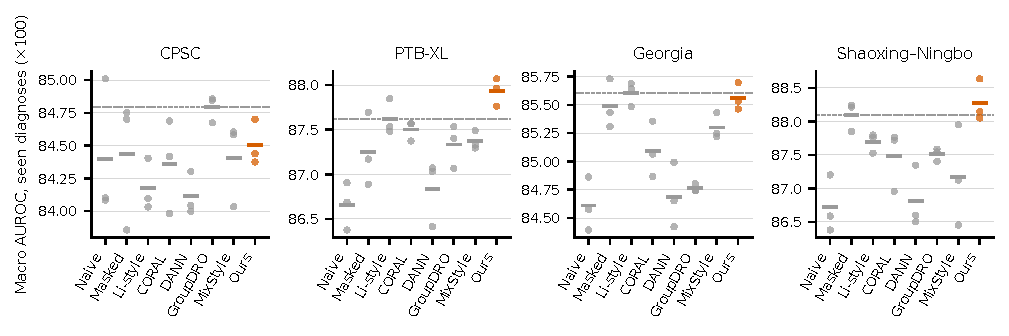
\includegraphics[width=\textwidth]{generated/fig_seen_seeds.pdf}
\caption{Seen-diagnosis macro AUROC of every run, per held-out database. Dots are individual seeds, horizontal bars the mean over three seeds; the dashed line marks the best baseline mean of each database. The proposed method (orange) has the highest mean on PTB-XL and Shaoxing--Ningbo, is level with the best baseline on Georgia, and lies within the spread of the baselines on CPSC.}\label{fig:seeds}
\end{figure}

The advantage is not uniform across databases. It is largest on PTB-XL ($87.9$ against $87.6$ for the best baseline) and Shaoxing--Ningbo ($88.3$ against $88.1$), where the mean of the proposed method exceeds that of every baseline (Fig.~
ef{fig:seeds}). On Georgia the proposed method ties with Li-style masking ($85.6$), and on CPSC it lies within the spread of the baselines, GroupDRO being highest ($84.8$ against $84.5$). CPSC is the held-out database with the smallest annotated vocabulary and the longest recordings, and GroupDRO, which up-weights the worst-performing source, is the only DG method that helps on it.

Table~\ref{tab:seedstats} gives the primary statistical analysis over the twelve paired fold--seed runs. For macro AUROC, the proposed method is better than every baseline in at least eight of twelve pairs; after Holm correction the difference is significant against six of the seven baselines (naive, Li-style, CORAL, DANN, GroupDRO and MixStyle; $p_{\mathrm{Holm}}\le0.014$) but not against the masked baseline (mean difference $+0.25$ points, eight of twelve pairs, $p=0.052$). For macro AUPRC, the difference is significant against naive pooling, CORAL, DANN and MixStyle, but not against masked loss, Li-style or GroupDRO. The proposed method therefore matches the strongest baseline on seen diagnoses and significantly improves on the domain-generalization methods, with an effect size of a few tenths of a point of AUROC; it does not establish a significant advantage over well-implemented masking. Because our pre-specified selection rule would have chosen the linear-scoring variant rather than mean-probability fusion (Section~\ref{sec:selection}), we also report that variant here: its mean seen-diagnosis AUROC is $86.06_{\pm0.19}$, 0.21 points below the Li-style baseline, and its unseen-diagnosis AUROC is the same as that of the selected configuration (Table~\ref{tab:ablation}). Under the pre-specified rule, the conclusion on seen diagnoses would therefore be ``on par with or slightly below the strongest baselines'' rather than ``on par with the strongest and significantly above the others''; all conclusions on unseen and removed diagnoses are unaffected.

\begin{table}[!htbp]
\centering\footnotesize
\setlength{\tabcolsep}{4pt}
\caption{Primary statistical comparison over the twelve paired runs (four held-out databases $\times$ three seeds) of seen-diagnosis macro AUROC and AUPRC ($\times100$): mean difference (ours $-$ baseline), number of pairs in which the proposed method is better, and the exact two-sided Wilcoxon signed-rank $p$, Holm-adjusted over the seven baselines within each metric. Bold: $p_{\mathrm{Holm}}<0.05$.}\label{tab:seedstats}
\begin{tabular}{lcccccc}
\toprule
 & \multicolumn{3}{c}{Macro AUROC} & \multicolumn{3}{c}{Macro AUPRC} \\
\cmidrule(lr){2-4}\cmidrule(lr){5-7}
Ours vs. & $\Delta$ & wins & $p_{\mathrm{Holm}}$ & $\Delta$ & wins & $p_{\mathrm{Holm}}$ \\
\midrule
Naive pooling & $+0.97$ & 11/12 & \textbf{0.009} & $+0.75$ & 9/12 & \textbf{0.049} \\
Masked loss & $+0.25$ & 8/12 & 0.052 & $+0.15$ & 7/12 & 0.380 \\
Li-style & $+0.30$ & 10/12 & \textbf{0.010} & $+0.23$ & 8/12 & 0.105 \\
CORAL & $+0.46$ & 11/12 & \textbf{0.009} & $+0.92$ & 12/12 & \textbf{0.003} \\
DANN & $+0.95$ & 12/12 & \textbf{0.003} & $+1.07$ & 12/12 & \textbf{0.003} \\
GroupDRO & $+0.47$ & 9/12 & \textbf{0.014} & $+0.71$ & 10/12 & 0.081 \\
MixStyle & $+0.51$ & 11/12 & \textbf{0.010} & $+0.79$ & 12/12 & \textbf{0.003} \\
\bottomrule
\end{tabular}
\end{table}

The within-fold bootstrap of Table~\ref{tab:stats} gives the same picture from the perspective of test-record sampling. Of the 28 comparisons of the seed-0 runs, 15 remain significant after Holm correction, all in favour of the proposed method: five on PTB-XL, four on Georgia and six on Shaoxing--Ningbo; no comparison is significant on CPSC, and none is significant in favour of a baseline. Against the masked baseline, the difference is significant on PTB-XL ($+0.9$ points, 95\% CI $[0.4,1.4]$) but not on the other three folds.

\IfFileExists{generated/tab_stats.tex}{\begin{sidewaystable}
\centering
\footnotesize
\setlength{\tabcolsep}{3pt}
\caption{Paired bootstrap (2000 resamples of test records) of the difference in macro AUROC ($\times 100$) between our method and each baseline (seed 0), with 95\% confidence interval and two-sided $p$ (Holm-adjusted over all comparisons in the table). Bottom: number of labels for which our method is significantly better / worse than the strongest baseline per target (DeLong test, Holm-adjusted $p<0.05$) out of all evaluated labels.}
\label{tab:stats}
\begin{tabular}{lcccccccc}
\toprule
 & \multicolumn{2}{c}{CPSC} & \multicolumn{2}{c}{PTB-XL} & \multicolumn{2}{c}{Georgia} & \multicolumn{2}{c}{Shaoxing-Ningbo} \\
\cmidrule(lr){2-3} \cmidrule(lr){4-5} \cmidrule(lr){6-7} \cmidrule(lr){8-9}
Ours vs. & $\Delta$ [95\% CI] & $p_\mathrm{Holm}$ & $\Delta$ [95\% CI] & $p_\mathrm{Holm}$ & $\Delta$ [95\% CI] & $p_\mathrm{Holm}$ & $\Delta$ [95\% CI] & $p_\mathrm{Holm}$ \\
\midrule
Naive (unknown = negative) & $+0.3$ [-0.3, 0.9] & 1.000 & $+0.9$ [0.5, 1.2] & 0.028 & $+0.8$ [0.5, 1.2] & 0.028 & $+0.9$ [0.6, 1.0] & 0.028 \\
Masked loss & $+0.6$ [-0.3, 1.3] & 1.000 & $+0.9$ [0.4, 1.4] & 0.028 & $-0.0$ [-0.3, 0.2] & 1.000 & $+0.2$ [0.0, 0.4] & 0.325 \\
Hierarchical mask (Li et al.) & $+0.4$ [-0.3, 1.1] & 1.000 & $+0.3$ [-0.0, 0.6] & 0.550 & $+0.2$ [-0.0, 0.4] & 0.550 & $+0.5$ [0.4, 0.7] & 0.028 \\
CORAL & $+0.5$ [-0.3, 1.2] & 1.000 & $+0.4$ [0.0, 0.8] & 0.325 & $+0.3$ [0.0, 0.6] & 0.325 & $+0.3$ [0.1, 0.5] & 0.032 \\
DANN & $+0.4$ [-0.4, 1.1] & 1.000 & $+1.3$ [0.9, 1.8] & 0.028 & $+1.3$ [1.0, 1.6] & 0.028 & $+1.5$ [1.2, 1.7] & 0.028 \\
GroupDRO & $-0.2$ [-1.1, 0.5] & 1.000 & $+0.7$ [0.3, 1.1] & 0.028 & $+0.9$ [0.6, 1.1] & 0.028 & $+0.5$ [0.3, 0.7] & 0.028 \\
MixStyle & $-0.2$ [-1.0, 0.5] & 1.000 & $+0.4$ [0.2, 0.7] & 0.032 & $+0.4$ [0.2, 0.7] & 0.042 & $+1.6$ [1.4, 1.8] & 0.028 \\
\midrule
DeLong vs.\ best & \multicolumn{2}{c}{GroupDRO: 3 / 1 of 23} & \multicolumn{2}{c}{Hierarchical mask (Li et al.): 1 / 4 of 32} & \multicolumn{2}{c}{Masked loss: 3 / 2 of 33} & \multicolumn{2}{c}{Masked loss: 7 / 5 of 36} \\
\bottomrule
\end{tabular}
\end{sidewaystable}
}{}

Table~\ref{tab:loso_f1} reports macro F1. At thresholds tuned on the source validation split all methods lie between $28.2$ and $29.7$ on average, and the proposed method ($29.4$) is not distinguishable from the best label-handling baselines; at the oracle threshold it obtains the highest mean F1 ($37.9$). The gap of about eight points between source-tuned and oracle F1, which is similar for all methods, shows that decision thresholds transfer poorly between databases whatever the training method, a point we return to in Section~\ref{sec:discussion}.

\IfFileExists{generated/tab_loso_f1.tex}{\begin{sidewaystable}
\centering
\footnotesize
\setlength{\tabcolsep}{3pt}
\caption{Leave-one-database-out macro F1 ($\times 100$) over seen labels, with thresholds tuned on source validation data (F1) and the oracle threshold on the target (F1$^{*}$, upper bound).}
\label{tab:loso_f1}
\begin{tabular}{lcccccccccc}
\toprule
 & \multicolumn{2}{c}{CPSC} & \multicolumn{2}{c}{PTB-XL} & \multicolumn{2}{c}{Georgia} & \multicolumn{2}{c}{Shaoxing-Ningbo} & \multicolumn{2}{c}{Mean} \\
\cmidrule(lr){2-3} \cmidrule(lr){4-5} \cmidrule(lr){6-7} \cmidrule(lr){8-9} \cmidrule(lr){10-11}
Method & F1 & F1$^{*}$ & F1 & F1$^{*}$ & F1 & F1$^{*}$ & F1 & F1$^{*}$ & F1 & F1$^{*}$ \\
\midrule
Naive (unknown = negative) & 23.4$_{\pm 0.4}$ & 32.1$_{\pm 0.3}$ & 31.2$_{\pm 0.6}$ & 41.5$_{\pm 0.3}$ & 32.1$_{\pm 0.6}$ & 41.1$_{\pm 0.4}$ & 26.1$_{\pm 0.5}$ & 33.5$_{\pm 0.4}$ & 28.2$_{\pm 0.4}$ & 37.1$_{\pm 0.1}$ \\
Masked loss & 23.8$_{\pm 0.1}$ & 32.6$_{\pm 0.2}$ & 32.4$_{\pm 0.7}$ & 42.2$_{\pm 0.2}$ & \textbf{33.4}$_{\pm 0.6}$ & \textbf{41.4}$_{\pm 0.1}$ & \textbf{28.3}$_{\pm 0.2}$ & 34.6$_{\pm 0.3}$ & 29.5$_{\pm 0.2}$ & 37.7$_{\pm 0.1}$ \\
Hierarchical mask (Li et al.) & 23.9$_{\pm 0.4}$ & 32.6$_{\pm 0.4}$ & 32.9$_{\pm 1.1}$ & 42.4$_{\pm 0.2}$ & 33.1$_{\pm 0.9}$ & 41.1$_{\pm 0.2}$ & 28.1$_{\pm 0.9}$ & 34.3$_{\pm 0.4}$ & 29.5$_{\pm 0.5}$ & 37.6$_{\pm 0.3}$ \\
CORAL & 23.7$_{\pm 0.5}$ & 31.7$_{\pm 0.2}$ & 32.8$_{\pm 0.8}$ & 42.1$_{\pm 0.3}$ & 33.0$_{\pm 0.5}$ & 40.0$_{\pm 0.4}$ & 27.5$_{\pm 0.3}$ & 34.1$_{\pm 0.7}$ & 29.3$_{\pm 0.2}$ & 37.0$_{\pm 0.2}$ \\
DANN & 23.8$_{\pm 0.5}$ & 31.8$_{\pm 0.4}$ & 32.7$_{\pm 1.2}$ & 41.8$_{\pm 0.3}$ & 33.3$_{\pm 1.0}$ & 39.9$_{\pm 0.4}$ & 26.8$_{\pm 0.8}$ & 33.3$_{\pm 0.1}$ & 29.2$_{\pm 0.4}$ & 36.7$_{\pm 0.2}$ \\
GroupDRO & \textbf{25.6}$_{\pm 0.4}$ & \textbf{33.3}$_{\pm 0.5}$ & \textbf{32.9}$_{\pm 0.7}$ & 41.1$_{\pm 0.4}$ & 32.0$_{\pm 0.3}$ & 38.9$_{\pm 0.1}$ & 28.2$_{\pm 0.5}$ & 34.4$_{\pm 0.3}$ & \textbf{29.7}$_{\pm 0.3}$ & 36.9$_{\pm 0.1}$ \\
MixStyle & 24.1$_{\pm 0.3}$ & 32.3$_{\pm 0.3}$ & 32.7$_{\pm 1.1}$ & 41.8$_{\pm 0.2}$ & 32.8$_{\pm 0.4}$ & 40.5$_{\pm 0.1}$ & 27.7$_{\pm 0.4}$ & 34.0$_{\pm 0.4}$ & 29.3$_{\pm 0.3}$ & 37.2$_{\pm 0.1}$ \\
\midrule
Ours & 23.8$_{\pm 0.4}$ & 33.1$_{\pm 0.5}$ & 32.9$_{\pm 0.2}$ & \textbf{42.5}$_{\pm 0.2}$ & 33.0$_{\pm 0.9}$ & 41.2$_{\pm 0.3}$ & 27.8$_{\pm 0.4}$ & \textbf{34.7}$_{\pm 0.5}$ & 29.4$_{\pm 0.2}$ & \textbf{37.9}$_{\pm 0.3}$ \\
\bottomrule
\end{tabular}
\end{sidewaystable}
}{}

\subsection{Unseen diagnoses}\label{sec:res_unseen}
Table~\ref{tab:unseen} and Fig.~\ref{fig:unseen} report the AUROC on diagnoses that only the held-out database annotates. On Shaoxing--Ningbo, where five diagnoses (left ventricular high voltage, clockwise and counterclockwise rotation, P-wave change and abnormal U wave) received no supervision of any kind, the proposed method obtains a macro AUROC of $67.0_{\pm1.3}$, against 51.2--53.2 for the seven baselines, whose untrained linear rows score at chance as expected. Four of the five diagnoses are scored clearly above chance by the text head: left ventricular high voltage ($71.3$, 5{,}401 positives), clockwise rotation ($73.3$), abnormal U wave ($74.8$) and P-wave change ($60.6$); counterclockwise rotation is close to chance ($54.9$). On CPSC the single unseen diagnosis, bradycardia, is implied by sinus bradycardia, so every method with implication completion has positive-only supervision for it; Li-style masking and the DG methods built on it reach 89.4--89.8 (CORAL 70.7, DANN 49.2), whereas the masked and naive baselines, which do not complete the label, remain at 48.0 and 64.6. The proposed method reaches $94.3_{\pm0.2}$, 4.5 points above the best baseline, which shows that the text anchor turns positive-only supervision into a well-ranked score where a linear row cannot.

\begin{table}[!htbp]
\centering\footnotesize
\setlength{\tabcolsep}{4pt}
\caption{AUROC ($\times100$) on diagnoses annotated only by the held-out database (unseen), mean$_{\pm\mathrm{std}}$ over three seeds. CPSC: bradycardia (1 diagnosis; supervised positive-only through implication completion by methods that use it). Shaoxing--Ningbo: macro AUROC over five diagnoses without any supervision. Linear-head baselines score unseen diagnoses with untrained or positive-only rows and serve as a chance reference.}\label{tab:unseen}
\begin{tabular}{lcc}
\toprule
Method & CPSC (Brady) & Shaoxing--Ningbo (5 diagnoses) \\
\midrule
Naive pooling & $64.6_{\pm1.2}$ & $53.2_{\pm4.6}$ \\
Masked loss & $48.0_{\pm1.3}$ & $52.1_{\pm1.5}$ \\
Li-style & $89.4_{\pm0.2}$ & $51.3_{\pm6.1}$ \\
CORAL & $70.7_{\pm4.4}$ & $51.8_{\pm0.6}$ \\
DANN & $49.2_{\pm12.7}$ & $52.6_{\pm3.0}$ \\
GroupDRO & $89.8_{\pm0.3}$ & $52.6_{\pm6.9}$ \\
MixStyle & $89.5_{\pm0.3}$ & $51.2_{\pm3.3}$ \\
\midrule
Ours (hybrid; text head on unseen) & $\mathbf{94.3}_{\pm0.2}$ & $\mathbf{67.0}_{\pm1.3}$ \\
\bottomrule
\end{tabular}
\end{table}

\begin{figure}[!htbp]
\centering
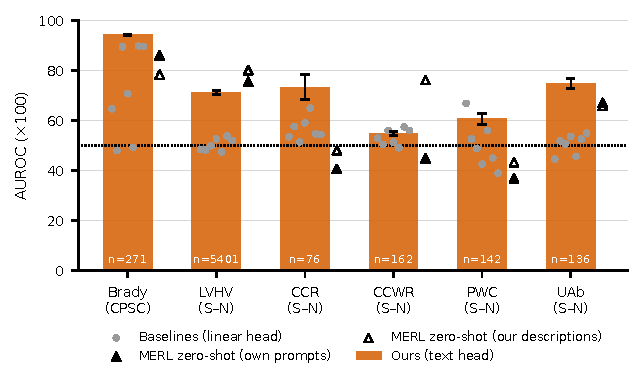
\includegraphics[width=0.75\textwidth]{generated/fig_unseen.pdf}
\caption{AUROC on each unseen diagnosis, mean over three seeds (bars, error bars one standard deviation) for the text head of the proposed method, and the seven linear-head baselines (grey dots). $n$ is the number of positive recordings in the held-out database. The dotted line marks chance. Abbreviations: Brady bradycardia; LVHV left ventricular high voltage; CCR, CCWR clockwise and counterclockwise cardiac rotation; PWC P-wave change; UAb abnormal U wave; S--N Shaoxing--Ningbo.}\label{fig:unseen}
\end{figure}

\subsection{Controlled annotation removal}\label{sec:res_e2}
Table~\ref{tab:e2} and Fig.~\ref{fig:e2} report the PTB-XL annotation-removal experiment. With complete annotation ($r=0$) the three methods are within 0.1 points of each other ($94.0$--$94.1$), confirming that the hybrid head does not cost in-distribution accuracy. When annotation is removed, the retained diagnoses degrade only mildly for all methods (at $r=0.5$: naive $92.6$, Li-style $91.3$, ours $93.1$). The removed diagnoses separate the methods. The linear baselines score them at or below chance: naive pooling $47.1$ and $55.5$ at $r=0.25$ and $0.5$, and Li-style $55.8$ and $47.6$, with large diagnosis-to-diagnosis variation that reflects the arbitrary orientation of untrained or negative-only rows. The proposed method scores them at $66.6$ and $69.0$, i.e.\ its open-vocabulary performance does not decline when the number of removed diagnoses grows from seven to seventeen. Per diagnosis at $r=0.5$ (Fig.~\ref{fig:e2}, right), the text head recovers conduction findings almost completely (right bundle branch block $93.5$, left anterior fascicular block $94.4$, first-degree AV block $78.2$, prolonged PR $73.8$), as well as atrial fibrillation ($77.2$) and flutter ($87.1$), T-wave inversion ($82.5$) and nonspecific ST--T abnormality ($82.1$). It fails on findings whose description is close to that of a related but different finding: sinus tachycardia ($43.6$), right axis deviation ($37.7$) and low QRS voltages ($49.6$). Over all diagnoses, removing annotation lowers the macro AUROC of the proposed method from $94.0$ to $79.5$ at $r=0.5$, against $71.6$ for naive pooling and $66.5$ for Li-style.

\begin{table}[!htbp]
\centering\footnotesize
\setlength{\tabcolsep}{5pt}
\caption{Controlled annotation removal on PTB-XL (single seed): macro AUROC ($\times100$) on the retained and the removed diagnoses and over all diagnoses, at removal rate $r$. At $r=0.25$ seven and at $r=0.5$ seventeen diagnoses are removed.}\label{tab:e2}
\begin{tabular}{lccccccc}
\toprule
 & $r=0$ & \multicolumn{3}{c}{$r=0.25$} & \multicolumn{3}{c}{$r=0.5$} \\
\cmidrule(lr){2-2}\cmidrule(lr){3-5}\cmidrule(lr){6-8}
Method & all & retained & removed & all & retained & removed & all \\
\midrule
Naive pooling & 94.1 & 93.2 & 47.1 & 82.5 & 92.6 & 55.5 & 71.6 \\
Li-style & 94.1 & 93.2 & 55.8 & 84.4 & 91.3 & 47.6 & 66.5 \\
Ours & 94.0 & 92.5 & \textbf{66.6} & \textbf{86.5} & \textbf{93.1} & \textbf{69.1} & \textbf{79.5} \\
\bottomrule
\end{tabular}
\end{table}

\begin{figure}[!htbp]
\centering
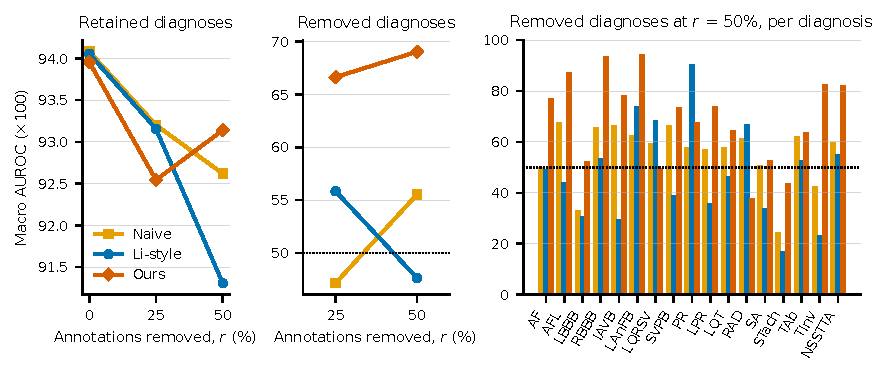
\includegraphics[width=\textwidth]{generated/fig_e2.pdf}
\caption{Controlled annotation removal on PTB-XL. Left and centre: macro AUROC on the retained and the removed diagnoses as a function of the fraction $r$ of PTB-XL diagnoses removed from training supervision. Right: AUROC on each of the seventeen diagnoses removed at $r=0.5$. The dotted line marks chance. Abbreviations follow Supplementary Table~S1.}\label{fig:e2}
\end{figure}

\subsection{Ablations}\label{sec:res_ablation}
Table~\ref{tab:ablation} and Fig.~\ref{fig:ablation} compare the selected configuration with the four variants of Section~\ref{sec:protocols}, all with three seeds, together with the Li-style baseline, which has the same label handling and encoder but no text head. Three observations follow. First, the gain on seen diagnoses comes from \emph{fusing} the two heads, not from the text head as an auxiliary task: scoring seen diagnoses by the linear head alone (linear scoring) gives $86.06$, slightly below the Li-style baseline ($86.27$), so jointly training the text head does not by itself improve the linear head. Second, joint training helps the fused model: the detached variant, which is a post-hoc ensemble of a Li-style encoder with a text head, reaches $86.43$, and letting the text-head gradient reach the encoder adds a further $0.14$ points ($86.57$), with the lowest seed variance of all configurations ($\pm0.07$). Third, adding pseudo-labels (86.38) and replacing the hybrid by the best text-only design (85.66) both reduce performance; the text-only model also scores unseen diagnoses worse ($62.0$ against $67.0$), so the linear head improves the text head through the shared encoder as well. All hybrid variants score unseen Shaoxing--Ningbo diagnoses between $66.5$ and $67.3$, so the unseen-diagnosis performance is a property of the text head and is robust to how seen diagnoses are scored.

\begin{table}[!htbp]
\centering\scriptsize
\setlength{\tabcolsep}{1pt}
\caption{Ablations of the hybrid model under leave-one-database-out (three seeds each): seen-diagnosis macro AUROC per held-out database and mean, mean AUPRC, and macro AUROC on the five unseen Shaoxing--Ningbo diagnoses ($\times100$, mean$_{\pm\mathrm{std}}$). The Li-style baseline has the same label handling and encoder without a text head.}\label{tab:ablation}
\begin{tabular}{lccccccc}
\toprule
 & \multicolumn{4}{c}{Seen AUROC} & \multicolumn{2}{c}{Seen, mean} & Unseen \\
\cmidrule(lr){2-5}\cmidrule(lr){6-7}\cmidrule(lr){8-8}
Configuration & CPSC & PTB-XL & Georgia & S--N & AUROC & AUPRC & S--N \\
\midrule
Li-style (no text head) & 84.2$_{\pm 0.2}$ & 87.6$_{\pm 0.2}$ & 85.6$_{\pm 0.1}$ & 87.7$_{\pm 0.1}$ & 86.27$_{\pm 0.15}$ & 32.8$_{\pm 0.3}$ & 51.3$_{\pm 6.1}$ \\
\textbf{Ours} (fusion) & 84.5$_{\pm 0.2}$ & 87.9$_{\pm 0.2}$ & 85.6$_{\pm 0.1}$ & \textbf{88.3}$_{\pm 0.3}$ & \textbf{86.57}$_{\pm 0.07}$ & \textbf{33.0}$_{\pm 0.2}$ & 67.0$_{\pm 1.3}$ \\
(i) Linear scoring & 84.3$_{\pm 0.2}$ & 87.4$_{\pm 0.1}$ & 85.2$_{\pm 0.2}$ & 87.4$_{\pm 0.6}$ & 86.06$_{\pm 0.19}$ & 32.4$_{\pm 0.3}$ & \textbf{67.3}$_{\pm 0.8}$ \\
(ii) Detached text head & 84.1$_{\pm 0.1}$ & \textbf{88.0}$_{\pm 0.2}$ & \textbf{85.7}$_{\pm 0.1}$ & 88.0$_{\pm 0.1}$ & 86.43$_{\pm 0.05}$ & 32.8$_{\pm 0.1}$ & 66.7$_{\pm 1.0}$ \\
(iii) + pseudo-labels & \textbf{84.6}$_{\pm 0.1}$ & 87.6$_{\pm 0.1}$ & 85.5$_{\pm 0.1}$ & 87.9$_{\pm 0.3}$ & 86.38$_{\pm 0.09}$ & 32.9$_{\pm 0.2}$ & 66.5$_{\pm 0.1}$ \\
(iv) Text head only & 83.9$_{\pm 0.2}$ & 86.6$_{\pm 0.0}$ & 84.8$_{\pm 0.6}$ & 87.3$_{\pm 0.1}$ & 85.66$_{\pm 0.19}$ & 32.0$_{\pm 0.2}$ & 62.0$_{\pm 1.7}$ \\
\bottomrule
\end{tabular}
\end{table}

\begin{figure}[!htbp]
\centering
\IfFileExists{generated/fig_ablation.pdf}{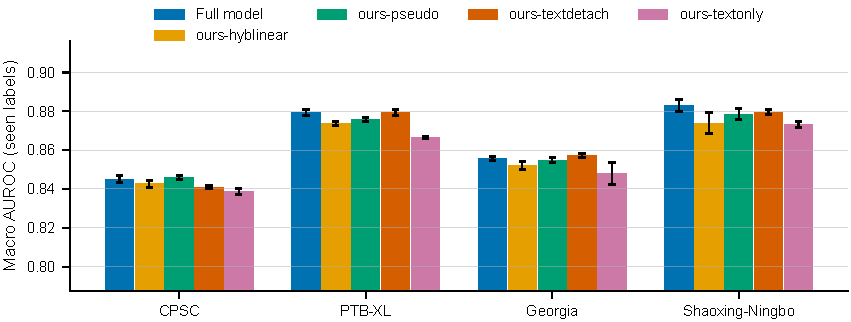
\includegraphics[width=\textwidth]{generated/fig_ablation.pdf}}{}
\caption{Seen-diagnosis macro AUROC of the selected configuration (``Full model'') and the four ablations per held-out database; bars are means over three seeds and error bars one standard deviation. ours-hyblinear: linear scoring; ours-textdetach: detached text head; ours-pseudo: with pseudo-labels; ours-textonly: text head only.}\label{fig:ablation}
\end{figure}

\subsection{Per-diagnosis analysis}\label{sec:res_perlabel}
Figure~\ref{fig:heatmap} shows, for each held-out database and each evaluable seen diagnosis, the AUROC difference between the proposed method and the strongest baseline of that database (seed 0), with DeLong tests Holm-corrected over all per-diagnosis comparisons; the bottom row of Table~\ref{tab:stats} counts the significant differences. The differences are small for most diagnoses and go in both directions: the proposed method is significantly better on 14 of 124 database--diagnosis pairs and significantly worse on 12, which is consistent with a two-head ensemble that redistributes rather than uniformly raises per-diagnosis accuracy. The largest gains are on conduction and morphology findings that share their description with related diagnoses (for example bundle branch block on Georgia, $+12.2$ points, and atrial flutter and nonspecific intraventricular conduction disorder on Shaoxing--Ningbo, $+5.7$ and $+6.6$), and the largest losses are on diagnoses defined by an absolute amplitude or interval that the description cannot convey precisely (low QRS voltages on Shaoxing--Ningbo, $-2.8$, and prolonged QT on Georgia, $-3.5$), and on bundle branch block on Shaoxing--Ningbo ($-7.8$). The sign of the bundle-branch-block difference thus depends on the database, which indicates that this parent finding is coded differently across sources.

\begin{figure}[!htbp]
\centering
\IfFileExists{generated/fig_perlabel_heatmap.pdf}{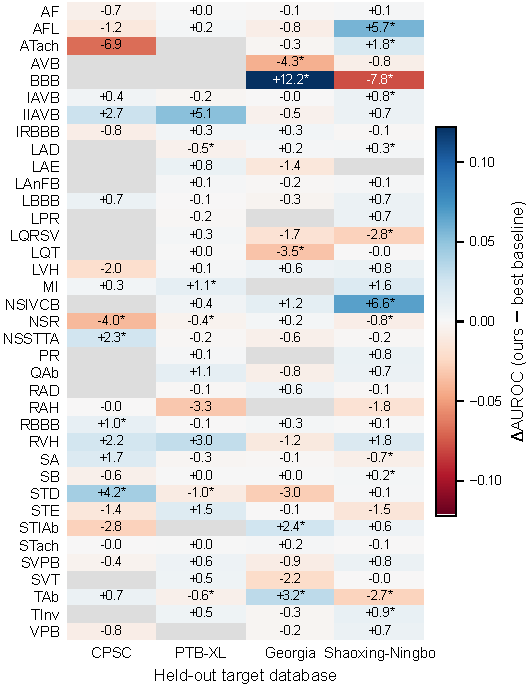
\includegraphics[width=\textwidth]{generated/fig_perlabel_heatmap.pdf}}{}
\caption{Per-diagnosis AUROC difference (proposed method $-$ strongest baseline of each held-out database, seed 0, $\times100$) on seen diagnoses. Marked cells are significant by DeLong's test after Holm correction over all per-diagnosis tests. Empty cells: diagnosis not evaluable in that database.}\label{fig:heatmap}
\end{figure}
